\PassOptionsToPackage{numbers}{natbib}
\documentclass{tufte-handout}
\usepackage{pgfplots}
\usepackage[dvipsnames]{xcolor}
\usepackage{amsmath, amssymb, amsthm}
\usepackage{mathtools}
\usepackage{bm}
\usepackage{thmtools}
\usepackage{enumitem}
\usepackage{graphicx}
\usepackage{caption}
\usepackage{subcaption}
\usepackage{tikz}
\usetikzlibrary{calc,arrows.meta,patterns}

% Color scheme (matching the original)
\definecolor{wp-bg}{HTML}{FDF6EF}
\definecolor{wp-text}{HTML}{2D1B0E}
\definecolor{wp-primary}{HTML}{C24A3A}
\definecolor{wp-accent}{HTML}{D4952E}
\definecolor{wp-light}{HTML}{F0DECA}
\definecolor{wp-muted}{HTML}{C4A88A}
\definecolor{wp-dark}{HTML}{1A0F07}

\pagecolor{wp-bg}
\color{wp-text}
\hypersetup{colorlinks=true,linkcolor=wp-primary,urlcolor=wp-accent}

% Theorem environments
\declaretheorem[style=plain, name=Definition, numberwithin=section]{defn}
\declaretheorem[style=plain, name=Theorem, numberwithin=section]{thm}
\declaretheorem[style=plain, name=Lemma, numberwithin=section]{lem}
\declaretheorem[style=remark, name=Example, numberwithin=section]{exmp}
\declaretheorem[style=remark, name=Remark, numberwithin=section]{remark}

\title{Foundations of Probability and Statistical Learning for Deep Learning}
\author{Vitor N. Cabral de Oliveira\\ \href{mailto:vnco@cin.ufpe.br}{vnco@cin.ufpe.br}}
\date{December 2024}

\begin{document}

\maketitle

\begin{abstract}
    These notes provide a self-contained mathematical foundation for deep learning, beginning with the axioms of probability theory, moving through random variables, expectation, limit theorems, multivariate distributions, and information theory. We then formalize the statistical learning framework: the learning problem, empirical risk minimization, bias–variance decomposition, and stochastic gradient descent. This combined foundation equips the reader with the rigorous tools needed to understand modern machine learning algorithms.
\end{abstract}

\newpage
\hypersetup{linkcolor=wp-text}
\tableofcontents
\hypersetup{linkcolor=wp-primary}
\newpage

\section{Probability Spaces and Axioms}

Probability theory begins with a mathematical model for random experiments. The fundamental structure is the \textbf{probability space}.

\begin{defn}[Probability Space]
    A probability space is a triple $(\Omega, \mathcal{F}, P)$ where:
    \begin{enumerate}[label=(\roman*)]
        \item $\Omega$ is a nonempty set, called the \textbf{sample space}. Its elements $\omega \in \Omega$ are elementary outcomes.
        \item $\mathcal{F}$ is a $\sigma$-\textbf{algebra} (or $\sigma$-field) of subsets of $\Omega$: a collection of subsets containing $\Omega$, closed under complement and countable union. The elements $A \in \mathcal{F}$ are called \textbf{events}.
        \item $P: \mathcal{F} \to [0,1]$ is a \textbf{probability measure} satisfying the Kolmogorov axioms:
            \begin{enumerate}
                \item $P(A) \ge 0$ for all $A \in \mathcal{F}$.
                \item $P(\Omega) = 1$.
                \item If $A_1, A_2, \dots$ are pairwise disjoint ($A_i \cap A_j = \varnothing$ for $i \ne j$), then
                \[
                P\!\left(\bigcup_{i=1}^{\infty} A_i\right) = \sum_{i=1}^{\infty} P(A_i) \quad \text{($\sigma$-additivity)}.
                \]
            \end{enumerate}
    \end{enumerate}
\end{defn}

\begin{marginfigure}
\centering
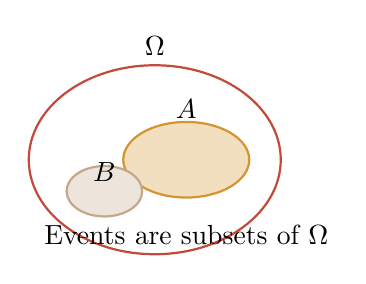
\begin{tikzpicture}[scale=0.8]
    \draw[thick, wp-primary] (0,0) ellipse (2 and 1.5);
    \node at (0,1.8) {$\Omega$};
    \fill[wp-accent!30, draw=wp-accent, thick] (0.5,0) ellipse (1 and 0.6);
    \node at (0.5,0.8) {$A$};
    \fill[wp-muted!30, draw=wp-muted, thick] (-0.8,-0.5) ellipse (0.6 and 0.4);
    \node at (-0.8,-0.2) {$B$};
    \node at (0.5,-1.2) {Events are subsets of $\Omega$};
\end{tikzpicture}
\caption{A sample space $\Omega$ with two events $A$ and $B$.}
\end{marginfigure}

The $\sigma$-algebra $\mathcal{F}$ formalizes which subsets of $\Omega$ are considered measurable (i.e., we can assign a probability). In discrete settings we often take $\mathcal{F} = 2^{\Omega}$ (all subsets). For continuous spaces like $\mathbb{R}$, we use the Borel $\sigma$-algebra generated by open intervals.

\subsection{Properties of Probability Measures}

From the axioms we derive several useful properties:
\begin{itemize}
    \item $P(\varnothing) = 0$.
    \item Finite additivity: for disjoint $A_1,\dots,A_n$, $P(\bigcup_{i=1}^n A_i) = \sum_{i=1}^n P(A_i)$.
    \item Monotonicity: If $A \subseteq B$, then $P(A) \le P(B)$.
    \item Complement: $P(A^c) = 1 - P(A)$.
    \item Union bound (Boole's inequality): $P(\bigcup_i A_i) \le \sum_i P(A_i)$.
    \item Inclusion–exclusion: $P(A \cup B) = P(A) + P(B) - P(A \cap B)$.
\end{itemize}

\subsection{Conditional Probability and Independence}

Conditional probability quantifies how the probability of an event changes given that another event has occurred.

\begin{defn}[Conditional Probability]
    For events $A$ and $B$ with $P(B) > 0$, the conditional probability of $A$ given $B$ is
    \[
    P(A \mid B) = \frac{P(A \cap B)}{P(B)}.
    \]
\end{defn}

\begin{defn}[Independence]
    Two events $A$ and $B$ are \textbf{independent} if $P(A \cap B) = P(A)P(B)$. Equivalently, $P(A \mid B) = P(A)$ when $P(B)>0$. A collection $\{A_i\}$ is mutually independent if for every finite subset $I$,
    \[
    P\!\left(\bigcap_{i \in I} A_i\right) = \prod_{i \in I} P(A_i).
    \]
\end{defn}

\paragraph{Bayes' Theorem}
A fundamental result that reverses conditioning:
\[
P(A \mid B) = \frac{P(B \mid A) P(A)}{P(B)}, \qquad \text{where } P(B) = \sum_i P(B \mid A_i)P(A_i)
\]
for a partition $\{A_i\}$ of $\Omega$. Bayes' theorem is the cornerstone of Bayesian inference and permeates modern machine learning (e.g., naive Bayes classifiers, Bayesian neural networks).

\begin{marginfigure}
\centering
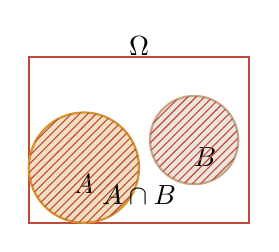
\begin{tikzpicture}[scale=0.7]
    \draw[thick, wp-primary] (0,0) rectangle (4,3);
    \node at (2,3.2) {$\Omega$};
    \fill[wp-accent!30, draw=wp-accent, thick] (1,1) circle (1);
    \node at (1,0.7) {$A$};
    \fill[wp-muted!30, draw=wp-muted, thick] (3,1.5) circle (0.8);
    \node at (3.2,1.2) {$B$};
    \fill[pattern=north east lines, pattern color=wp-primary] (1,1) circle (1) (3,1.5) circle (0.8);
    \node at (2,0.5) {$A \cap B$};
\end{tikzpicture}
\caption{Bayes' theorem relates $P(A|B)$ to $P(B|A)$ via the prior $P(A)$ and evidence $P(B)$.}
\end{marginfigure}

\section{Random Variables}

Often we are not directly interested in elementary outcomes but in numerical quantities derived from them.

\begin{defn}[Random Variable]
    A \textbf{random variable} $X$ on a probability space $(\Omega,\mathcal{F},P)$ is a function $X: \Omega \to \mathbb{R}$ such that for every Borel set $B \subseteq \mathbb{R}$, the preimage $X^{-1}(B) = \{\omega: X(\omega) \in B\}$ belongs to $\mathcal{F}$ (i.e., $X$ is \textit{measurable}). This condition ensures that probabilities of events involving $X$ are well-defined.
\end{defn}

\subsection{Discrete and Continuous Random Variables}

\begin{itemize}
    \item \textbf{Discrete} $X$ takes values in a countable set $\mathcal{X} \subseteq \mathbb{R}$. It is described by its \textbf{probability mass function (PMF)} $p_X(x) = P(X = x)$.
    \item \textbf{Continuous} $X$ has a \textbf{probability density function (PDF)} $f_X(x)$ such that for any interval $[a,b]$,
    \[
    P(a \le X \le b) = \int_a^b f_X(x)\,dx.
    \]
    The PDF satisfies $f_X(x) \ge 0$ and $\int_{-\infty}^{\infty} f_X(x)\,dx = 1$.
\end{itemize}

The \textbf{cumulative distribution function (CDF)} $F_X(x) = P(X \le x)$ is defined for any random variable and is non‑decreasing, right‑continuous, with $\lim_{x\to-\infty}F_X(x)=0$, $\lim_{x\to\infty}F_X(x)=1$.

\begin{marginfigure}
\centering
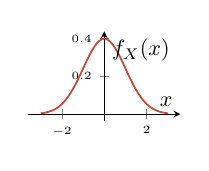
\begin{tikzpicture}[scale=0.8]
    \begin{axis}[width=4cm, height=3cm, xlabel=$x$, ylabel=$f_X(x)$, domain=-3:3, samples=100, axis lines=middle, enlargelimits, ticklabel style={font=\tiny}]
        \addplot[wp-primary, thick] {exp(-x^2/2)/sqrt(2*pi)};
    \end{axis}
\end{tikzpicture}
\caption{PDF of the standard normal distribution.}
\end{marginfigure}

\section{Expectation and Moments}

The expectation (mean) is the weighted average of a random variable.

\begin{defn}[Expectation]
    For a discrete random variable $X$ with PMF $p_X$, $\mathbb{E}[X] = \sum_{x} x\, p_X(x)$ (provided the sum converges absolutely). For continuous $X$ with PDF $f_X$, $\mathbb{E}[X] = \int_{-\infty}^{\infty} x\, f_X(x)\,dx$.
\end{defn}

\paragraph{Properties of Expectation}
\begin{itemize}
    \item Linearity: $\mathbb{E}[aX + bY] = a\mathbb{E}[X] + b\mathbb{E}[Y]$ for constants $a,b$.
    \item If $X \ge 0$ almost surely, then $\mathbb{E}[X] \ge 0$.
    \item Law of the unconscious statistician: $\mathbb{E}[g(X)] = \sum_x g(x)p_X(x)$ (discrete) or $\int g(x)f_X(x)\,dx$ (continuous).
\end{itemize}

\subsection{Variance and Covariance}

\begin{defn}[Variance]
    The variance of $X$ measures its spread around the mean:
    \[
    \operatorname{Var}(X) = \mathbb{E}\bigl[(X - \mathbb{E}[X])^2\bigr] = \mathbb{E}[X^2] - (\mathbb{E}[X])^2.
    \]
    The standard deviation is $\sigma_X = \sqrt{\operatorname{Var}(X)}$.
\end{defn}

\begin{defn}[Covariance and Correlation]
    For two random variables $X,Y$,
    \[
    \operatorname{Cov}(X,Y) = \mathbb{E}\bigl[(X - \mathbb{E}[X])(Y - \mathbb{E}[Y])\bigr] = \mathbb{E}[XY] - \mathbb{E}[X]\mathbb{E}[Y].
    \]
    The correlation coefficient is $\rho(X,Y) = \frac{\operatorname{Cov}(X,Y)}{\sigma_X \sigma_Y}$, satisfying $-1 \le \rho \le 1$.
\end{defn}

If $X$ and $Y$ are independent, then $\operatorname{Cov}(X,Y)=0$ (the converse is not true in general).

\section{Important Distributions for Machine Learning}

Several probability distributions appear repeatedly in machine learning.

\subsection{Bernoulli and Binomial}
\begin{itemize}
    \item \textbf{Bernoulli}$(\theta)$: $X \in \{0,1\}$, $P(X=1)=\theta$, $P(X=0)=1-\theta$. $\mathbb{E}[X]=\theta$, $\operatorname{Var}(X)=\theta(1-\theta)$. Used for binary classification.
    \item \textbf{Binomial}$(n,\theta)$: $X = \sum_{i=1}^n Y_i$ with $Y_i$ i.i.d. Bernoulli$(\theta)$. PMF: $P(X=k) = \binom{n}{k}\theta^k(1-\theta)^{n-k}$, $\mathbb{E}[X]=n\theta$, $\operatorname{Var}(X)=n\theta(1-\theta)$.
\end{itemize}

\subsection{Gaussian (Normal) Distribution}
The most ubiquitous continuous distribution.
\[
\mathcal{N}(\mu, \sigma^2):\quad f(x) = \frac{1}{\sqrt{2\pi\sigma^2}} \exp\!\left(-\frac{(x-\mu)^2}{2\sigma^2}\right),\quad \mathbb{E}[X]=\mu,\ \operatorname{Var}(X)=\sigma^2.
\]
The standard normal $\mathcal{N}(0,1)$ has mean $0$ and variance $1$. By the Central Limit Theorem, sums of many independent random variables tend to a Gaussian.

\subsection{Exponential and Laplace}
\begin{itemize}
    \item \textbf{Exponential}$(\lambda)$: $f(x) = \lambda e^{-\lambda x}$, $x \ge 0$, $\mathbb{E}[X]=1/\lambda$. Used for waiting times.
    \item \textbf{Laplace}$(\mu,b)$: $f(x) = \frac{1}{2b}\exp\!\left(-\frac{|x-\mu|}{b}\right)$. Heavier tails than Gaussian; used in robust regression.
\end{itemize}

\subsection{Multivariate Gaussian}
For a random vector $\mathbf{X} = (X_1,\dots,X_d)^{\mathsf{T}}$,
\[
\mathcal{N}(\boldsymbol{\mu}, \boldsymbol{\Sigma}):\quad f(\mathbf{x}) = \frac{1}{(2\pi)^{d/2}|\boldsymbol{\Sigma}|^{1/2}} \exp\!\left(-\frac{1}{2}(\mathbf{x}-\boldsymbol{\mu})^{\mathsf{T}}\boldsymbol{\Sigma}^{-1}(\mathbf{x}-\boldsymbol{\mu})\right),
\]
with mean vector $\boldsymbol{\mu} \in \mathbb{R}^d$ and positive‑definite covariance matrix $\boldsymbol{\Sigma}$. This is the foundation of many latent variable models and deep generative models (e.g., variational autoencoders).

\section{Limit Theorems}

These theorems justify why averaging works and why the Gaussian distribution appears so often.

\begin{thm}[Law of Large Numbers (LLN)]
    Let $X_1, X_2, \dots$ be i.i.d. with $\mathbb{E}[X_i] = \mu$. Then the sample average $\overline{X}_n = \frac{1}{n}\sum_{i=1}^n X_i$ converges to $\mu$ in probability:
    \[
    \forall \varepsilon >0,\quad \lim_{n\to\infty} P(|\overline{X}_n - \mu| > \varepsilon) = 0.
    \]
\end{thm}

\begin{thm}[Central Limit Theorem (CLT)]
    Under the same i.i.d. assumption with finite variance $\sigma^2$, the scaled sample average converges in distribution to a standard normal:
    \[
    \sqrt{n}\,\frac{\overline{X}_n - \mu}{\sigma} \xrightarrow{d} \mathcal{N}(0,1).
    \]
    Equivalently, $\overline{X}_n \approx \mathcal{N}(\mu, \sigma^2/n)$ for large $n$.
\end{thm}

\begin{marginfigure}
\centering
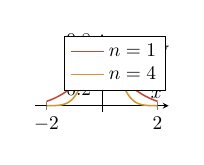
\begin{tikzpicture}[scale=0.7]
    \begin{axis}[width=4cm, height=3cm, xlabel=$\overline{x}$, ylabel=density, domain=-2:2, samples=100, axis lines=middle, enlargelimits]
        \addplot[wp-primary, thick] {exp(-x^2/2)/sqrt(2*pi)};
        \addplot[wp-accent, thick, domain=-2:2] {exp(-x^2/(2*0.25))/sqrt(2*pi*0.25)};
        \legend{$n=1$, $n=4$};
    \end{axis}
\end{tikzpicture}
\caption{The CLT: as $n$ increases, the distribution of $\overline{X}_n$ becomes narrower and more Gaussian.}
\end{marginfigure}

The CLT explains why the Gaussian prior is a common choice and why many estimators are asymptotically normal.

\section{Multivariate Random Vectors and Joint Distributions}

When dealing with multiple random variables simultaneously, we use the joint distribution.

\begin{defn}[Joint PDF/PMF]
    For a random vector $(X_1,\dots,X_d)$:
    \begin{itemize}
        \item Discrete: joint PMF $p(x_1,\dots,x_d) = P(X_1=x_1,\dots,X_d=x_d)$.
        \item Continuous: joint PDF $f(x_1,\dots,x_d)$ satisfying $P(\mathbf{X} \in A) = \int_A f(\mathbf{x})\,d\mathbf{x}$.
    \end{itemize}
\end{defn}

\subsection{Marginal and Conditional Distributions}
\begin{itemize}
    \item \textbf{Marginal} PMF/PDF: e.g., $p_{X_1}(x_1) = \sum_{x_2,\dots,x_d} p(x_1,\dots,x_d)$ (discrete) or $f_{X_1}(x_1) = \int \cdots \int f(x_1,\dots,x_d)\,dx_2\cdots dx_d$ (continuous).
    \item \textbf{Conditional} distribution of $X$ given $Y=y$: $f_{X|Y}(x|y) = \frac{f_{X,Y}(x,y)}{f_Y(y)}$ (for continuous) and similarly for PMF.
\end{itemize}

\subsection{Independence of Random Variables}
Random variables $X_1,\dots,X_d$ are independent iff their joint distribution factorizes:
\[
f(x_1,\dots,x_d) = \prod_{i=1}^d f_{X_i}(x_i) \quad (\text{or PMF analog}).
\]
Independence simplifies many computations and is a common modeling assumption (e.g., naive Bayes).

\subsection{Law of Total Expectation and Variance}
For two random variables $X,Y$,
\[
\mathbb{E}[X] = \mathbb{E}\bigl[\mathbb{E}[X \mid Y]\bigr],\qquad
\operatorname{Var}(X) = \mathbb{E}\bigl[\operatorname{Var}(X \mid Y)\bigr] + \operatorname{Var}\bigl(\mathbb{E}[X \mid Y]\bigr).
\]
These identities are crucial in deriving algorithms like expectation–maximization and in analyzing stochastic gradient descent.

\section{Information Theory for Machine Learning}

Information theory provides a rigorous framework for quantifying uncertainty, information, and dependence between random variables. These concepts are indispensable in machine learning: they underlie loss functions (cross‑entropy), regularization (mutual information bottleneck), and evaluation metrics (KL divergence for distribution matching). Building on the probability foundations developed earlier, we now introduce the core quantities of information theory.

\subsection{Entropy: Quantifying Uncertainty}

\begin{defn}[Shannon Entropy]
    For a discrete random variable $X$ with probability mass function $p(x) = P(X=x)$, the \textbf{entropy} $H(X)$ is defined as
    \[
    H(X) = -\sum_{x \in \mathcal{X}} p(x) \log p(x),
    \]
    with the convention $0 \log 0 = 0$. The logarithm is typically taken base 2 (giving units of \textit{bits}) or base $e$ (natural units, \textit{nats}). Entropy measures the average uncertainty about the outcome of $X$.
\end{defn}

\begin{marginfigure}
\centering
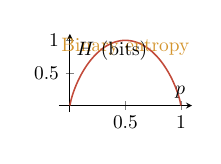
\begin{tikzpicture}[scale=0.7]
    \begin{axis}[width=4cm, height=3cm, xlabel=$p$, ylabel=$H$ (bits), domain=0:1, samples=100, axis lines=middle, enlargelimits]
        \addplot[wp-primary, thick] {-x*log2(x) - (1-x)*log2(1-x)};
        \node[wp-accent] at (0.5, 0.9) {Binary entropy};
    \end{axis}
\end{tikzpicture}
\caption{Binary entropy $H(p) = -p\log_2 p - (1-p)\log_2(1-p)$. Maximum uncertainty at $p=0.5$.}
\end{marginfigure}

\paragraph{Properties of Entropy}
\begin{itemize}
    \item $H(X) \ge 0$, with equality iff $X$ is deterministic ($p(x)=1$ for some $x$).
    \item For a uniform distribution over $m$ outcomes, $H(X) = \log m$ (maximum entropy given finite support).
    \item For independent random variables, $H(X,Y) = H(X) + H(Y)$.
\end{itemize}

\subsection{Joint and Conditional Entropy}

\begin{defn}[Joint Entropy]
    For two discrete random variables $X$ and $Y$ with joint PMF $p(x,y)$,
    \[
    H(X,Y) = -\sum_{x \in \mathcal{X}} \sum_{y \in \mathcal{Y}} p(x,y) \log p(x,y).
    \]
\end{defn}

\begin{defn}[Conditional Entropy]
    The conditional entropy $H(Y \mid X)$ is the average uncertainty about $Y$ given knowledge of $X$:
    \[
    H(Y \mid X) = \sum_{x} p(x) \, H(Y \mid X=x) = -\sum_{x,y} p(x,y) \log p(y \mid x).
    \]
\end{defn}

\paragraph{Chain Rule for Entropy}
\[
H(X,Y) = H(X) + H(Y \mid X) = H(Y) + H(X \mid Y).
\]
This mirrors the product rule of probabilities.

\subsection{Mutual Information}

Mutual information quantifies the amount of information that one random variable contains about another.

\begin{defn}[Mutual Information]
    The mutual information between $X$ and $Y$ is
    \[
    I(X;Y) = H(X) - H(X \mid Y) = H(Y) - H(Y \mid X) = H(X) + H(Y) - H(X,Y).
    \]
    Equivalently,
    \[
    I(X;Y) = \sum_{x,y} p(x,y) \log \frac{p(x,y)}{p(x)p(y)} = D_{\text{KL}}(P_{XY} \parallel P_X P_Y).
    \]
\end{defn}

\begin{marginfigure}
\centering
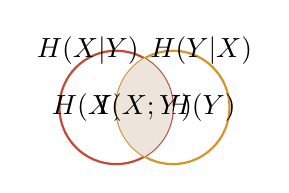
\begin{tikzpicture}[scale=0.6]
    \draw[wp-primary, thick] (0,0) circle (1.2);
    \draw[wp-accent, thick] (1.2,0) circle (1.2);
    \node at (-0.6,0) {$H(X)$};
    \node at (1.8,0) {$H(Y)$};
    \begin{scope}
        \clip (0,0) circle (1.2);
        \fill[wp-muted!30] (1.2,0) circle (1.2);
    \end{scope}
    \node at (0.6,0) {$I(X;Y)$};
    \node at (-0.6,1.2) {$H(X|Y)$};
    \node at (1.8,1.2) {$H(Y|X)$};
\end{tikzpicture}
\caption{Venn diagram interpretation: mutual information is the intersection of information content.}
\end{marginfigure}

\paragraph{Properties of Mutual Information}
\begin{itemize}
    \item $I(X;Y) \ge 0$, with equality iff $X$ and $Y$ are independent.
    \item $I(X;Y) = I(Y;X)$ (symmetry).
    \item $I(X;Y) \le \min(H(X), H(Y))$.
    \item Invariant under invertible transformations (e.g., scaling, bijections).
\end{itemize}

Mutual information is central to representation learning (e.g., InfoGAN, contrastive learning) and to the information bottleneck principle for deep learning.

\subsection{Kullback–Leibler Divergence}

The KL divergence measures how one probability distribution diverges from another.

\begin{defn}[Kullback–Leibler Divergence]
    For two discrete distributions $p$ and $q$ over the same alphabet $\mathcal{X}$,
    \[
    D_{\text{KL}}(p \parallel q) = \sum_{x \in \mathcal{X}} p(x) \log \frac{p(x)}{q(x)},
    \]
    with $0 \log 0 = 0$ and $p(x) \log 0 = \infty$ if $p(x) > 0$ and $q(x)=0$. It satisfies $D_{\text{KL}}(p \parallel q) \ge 0$, with equality iff $p = q$ almost everywhere.
\end{defn}

\begin{remark}
    KL divergence is not a metric because it is asymmetric and does not satisfy the triangle inequality. Nonetheless it is the fundamental quantity in variational inference, expectation‑maximization, and generative modeling (e.g., VAEs minimize a KL term).
\end{remark}

\subsection{Cross‑Entropy}

Cross‑entropy is intimately related to KL divergence and appears directly as a loss function in classification.

\begin{defn}[Cross‑Entropy]
    The cross‑entropy between a true distribution $p$ and an approximation $q$ is
    \[
    H(p,q) = -\sum_{x} p(x) \log q(x) = H(p) + D_{\text{KL}}(p \parallel q).
    \]
\end{defn}

When $p$ is the empirical distribution of labels (e.g., one‑hot encoded) and $q$ is the model's predicted probability distribution (e.g., softmax output), minimizing cross‑entropy is equivalent to minimizing KL divergence (since $H(p)$ is constant with respect to the model). This is why categorical cross‑entropy is the standard loss for multi‑class classification.

\begin{marginfigure}
\centering
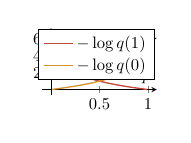
\begin{tikzpicture}[scale=0.6]
    \begin{axis}[width=4cm, height=3cm, xlabel=$p$, ylabel={Cross‑entropy}, domain=0.01:0.99, samples=100, axis lines=middle, enlargelimits]
        \addplot[wp-primary, thick] {-log2(x)};
        \addplot[wp-accent, thick] {-log2(1-x)};
        \legend{$-\log q(1)$, $-\log q(0)$};
    \end{axis}
\end{tikzpicture}
\caption{Cross‑entropy loss for binary classification: $-\log q(y)$ penalizes confident wrong predictions.}
\end{marginfigure}

\subsection{Differential Entropy for Continuous Variables}

For continuous random variables, entropy is replaced by \textbf{differential entropy}.

\begin{defn}[Differential Entropy]
    For a continuous random variable $X$ with PDF $f(x)$,
    \[
    h(X) = -\int_{\mathcal{X}} f(x) \log f(x)\,dx,
    \]
    provided the integral exists.
\end{defn}

\begin{remark}
    Unlike discrete entropy, differential entropy can be negative and is not invariant under coordinate transformations. However, mutual information $I(X;Y)$ remains well‑defined for continuous variables and inherits the same properties.
\end{remark}

\paragraph{Example: Gaussian Differential Entropy}
For $X \sim \mathcal{N}(\mu, \sigma^2)$,
\[
h(X) = \frac{1}{2} \log(2\pi e \sigma^2) \quad \text{(nats)}.
\]
This shows that the entropy increases with variance, as expected.

\subsection{Applications in Machine Learning}

\begin{itemize}
    \item \textbf{Classification losses:} Cross‑entropy loss directly derived from MLE under a categorical distribution.
    \item \textbf{Regularization:} Adding $D_{\text{KL}}(q \parallel p)$ as a penalty enforces a prior distribution on latent variables (e.g., in VAEs).
    \item \textbf{Feature selection:} Maximizing mutual information between features and labels while minimizing redundancy (minimum redundancy – maximum relevance, mRMR).
    \item \textbf{Information bottleneck:} Find a representation $Z$ that minimizes $I(X;Z) - \beta I(Z;Y)$, compressing $X$ while preserving information about $Y$.
    \item \textbf{Contrastive learning:} Mutual information estimation between augmented views of the same data point.
    \item \textbf{Generative models:} GANs implicitly minimize a divergence (Jensen–Shannon, Wasserstein), while VAEs explicitly minimize a KL term.
\end{itemize}

\begin{marginfigure}
\centering
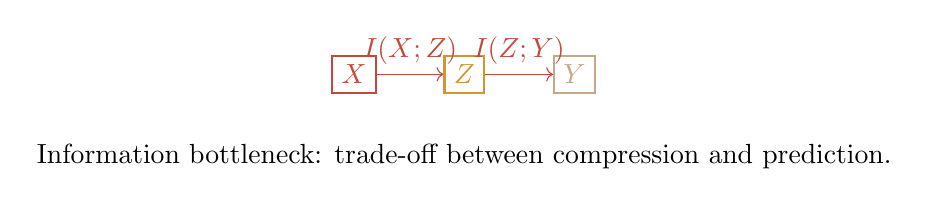
\begin{tikzpicture}[scale=0.7]
    \node[draw, wp-primary, thick, rectangle] (X) at (0,0) {$X$};
    \node[draw, wp-accent, thick, rectangle] (Z) at (2,0) {$Z$};
    \node[draw, wp-muted, thick, rectangle] (Y) at (4,0) {$Y$};
    \draw[->, wp-primary] (X) -- (Z) node[midway, above] {$I(X;Z)$};
    \draw[->, wp-primary] (Z) -- (Y) node[midway, above] {$I(Z;Y)$};
    \node at (2,-1.5) {Information bottleneck: trade‑off between compression and prediction.};
\end{tikzpicture}
\caption{Information bottleneck curve: find $Z$ maximizing $I(Z;Y)$ while minimizing $I(X;Z)$.}
\end{marginfigure}

With these information‑theoretic tools, we now have a complete probabilistic and statistical foundation that connects directly to deep learning objectives, regularization schemes, and evaluation criteria.

\section{Preliminary Foundations of Statistical Learning}

Armed with the probability theory developed above, we now formalize the problem of learning from data, which provides the theoretical basis for algorithms such as the perceptron and multilayer networks.

\subsection{The Learning Problem}

In supervised learning, we are given a training set $\mathcal{D} = \{(\mathbf{x}_i, y_i)\}_{i=1}^{N}$, where each $\mathbf{x}_i \in \mathcal{X} \subseteq \mathbb{R}^d$ is an input vector (feature vector) and $y_i \in \mathcal{Y}$ is the corresponding target output. The nature of $\mathcal{Y}$ defines the task:
\begin{itemize}
    \item \textbf{Classification:} $\mathcal{Y} = \{1,\dots, K\}$ (finite set of class labels).
    \item \textbf{Regression:} $\mathcal{Y} = \mathbb{R}$ (real-valued output).
\end{itemize}

The fundamental assumption is that the training examples are drawn independently and identically distributed (i.i.d.) from an unknown joint probability distribution $P(\mathbf{x}, y)$ over $\mathcal{X} \times \mathcal{Y}$.

\subsection{Hypothesis Space and Loss Functions}

A learning algorithm selects a hypothesis $h: \mathcal{X} \to \mathcal{Y}$ from a predefined hypothesis space $\mathcal{H}$. The quality of a hypothesis is measured by a \textbf{loss function} $\ell: \mathcal{Y} \times \mathcal{Y} \to \mathbb{R}_{\ge 0}$, where $\ell(h(\mathbf{x}), y)$ quantifies the cost of predicting $h(\mathbf{x})$ when the true target is $y$. Common loss functions include:
\begin{itemize}
    \item \textbf{0–1 loss (classification):} $\ell(h(\mathbf{x}), y) = \mathbf{1}_{h(\mathbf{x}) \neq y}$.
    \item \textbf{Squared loss (regression):} $\ell(h(\mathbf{x}), y) = (y - h(\mathbf{x}))^2$.
    \item \textbf{Cross-entropy loss (classification with probabilities):} $\ell(\hat{\mathbf{p}}, y) = -\sum_{k=1}^K \mathbf{1}_{y=k} \log \hat{p}_k$.
\end{itemize}

The ultimate goal is to minimize the \textbf{expected risk} (also called true risk or generalization error):
\begin{equation}
    R(h) = \mathbb{E}_{(\mathbf{x}, y) \sim P} \left[ \ell(h(\mathbf{x}), y) \right].
\end{equation}
Since $P$ is unknown, we cannot directly compute $R(h)$. Instead, we minimize the \textbf{empirical risk} over the training set:
\begin{equation}
    \widehat{R}_{\mathcal{D}}(h) = \frac{1}{N} \sum_{i=1}^{N} \ell(h(\mathbf{x}_i), y_i).
\end{equation}

\subsection{Empirical Risk Minimization (ERM)}

The principle of empirical risk minimization (ERM) selects the hypothesis that minimizes the empirical risk:
\begin{equation}
    h_{\text{ERM}} = \arg\min_{h \in \mathcal{H}} \widehat{R}_{\mathcal{D}}(h).
\end{equation}
For finite $\mathcal{H}$, uniform convergence bounds (e.g., Hoeffding's inequality together with union bound) guarantee that with high probability, $R(h_{\text{ERM}})$ is close to the minimal possible risk $\min_{h \in \mathcal{H}} R(h)$, provided the sample size $N$ is sufficiently large relative to the complexity of $\mathcal{H}$. This interplay between approximation error (bias) and estimation error (variance) is captured by the \textbf{bias–variance decomposition} (for squared loss):
\begin{equation}
    \mathbb{E}_{\mathcal{D}} \left[ R(h_{\mathcal{D}}) \right] = \underbrace{R(h^*)}_{\text{irreducible error}} + \underbrace{\left( \mathbb{E}_{\mathcal{D}}[h_{\mathcal{D}}] - h^* \right)^2}_{\text{bias}^2} + \underbrace{\mathbb{V}_{\mathcal{D}}[h_{\mathcal{D}}]}_{\text{variance}}.
\end{equation}
where $h^*$ is the Bayes-optimal hypothesis. Larger hypothesis spaces reduce bias but increase variance, leading to the classic \textbf{bias–variance tradeoff}.

\subsection{Stochastic Gradient Descent as an Optimization Method}

Most modern machine learning models, including neural networks, are trained by minimizing the empirical risk using gradient-based optimization. Because the empirical risk is an average over $N$ terms,
\[
\widehat{R}_{\mathcal{D}}(\mathbf{w}) = \frac{1}{N} \sum_{i=1}^N \ell_i(\mathbf{w}),
\]
the full gradient $\nabla \widehat{R}_{\mathcal{D}}(\mathbf{w})$ requires a pass through the entire dataset, which is computationally expensive for large $N$. The stochastic gradient descent (SGD) algorithm replaces the true gradient by an unbiased estimate computed from a mini‑batch of examples:
\[
\mathbf{w}_{t+1} = \mathbf{w}_t - \eta_t \cdot \frac{1}{|\mathcal{B}|} \sum_{i \in \mathcal{B}} \nabla \ell_i(\mathbf{w}_t),
\]
where $\mathcal{B} \subset \{1,\dots,N\}$ is a random mini‑batch. This stochastic approximation introduces noise but enables efficient optimisation, especially for large‑scale problems.

With these foundations in place, we can now proceed to study artificial neural networks, starting with the perceptron and leading to deep learning architectures.

\section{Maximum Likelihood Estimation and Bayesian Inference}

The statistical learning framework introduced above relies on minimizing empirical risk. However, a deeper probabilistic interpretation arises from \textbf{maximum likelihood estimation (MLE)} and \textbf{Bayesian inference}. These approaches explicitly model the data-generating distribution and provide a principled way to estimate parameters, quantify uncertainty, and incorporate prior knowledge.

\subsection{The Likelihood Function}

Assume we have a parametric family of distributions $\{P_{\boldsymbol{\theta}} : \boldsymbol{\theta} \in \Theta\}$ over the data space $\mathcal{X} \times \mathcal{Y}$ (or simply over $\mathcal{X}$ in unsupervised settings). Given i.i.d. observations $\mathcal{D} = \{(\mathbf{x}_i, y_i)\}_{i=1}^{N}$, the joint probability (or density) of the data as a function of $\boldsymbol{\theta}$ is the \textbf{likelihood}:
\[
L(\boldsymbol{\theta}; \mathcal{D}) = \prod_{i=1}^{N} p_{\boldsymbol{\theta}}(\mathbf{x}_i, y_i),
\]
where $p_{\boldsymbol{\theta}}$ denotes the PMF (discrete) or PDF (continuous). For supervised learning it is often convenient to factor the likelihood using the conditional distribution of $y$ given $\mathbf{x}$:
\[
L(\boldsymbol{\theta}; \mathcal{D}) = \prod_{i=1}^{N} p_{\boldsymbol{\theta}}(y_i \mid \mathbf{x}_i) \, p_{\boldsymbol{\theta}}(\mathbf{x}_i).
\]
If the marginal $p_{\boldsymbol{\theta}}(\mathbf{x})$ does not depend on $\boldsymbol{\theta}$ (or is ignored), we work with the conditional likelihood.

\subsection{Maximum Likelihood Estimation}

\begin{defn}[Maximum Likelihood Estimator]
    The maximum likelihood estimator (MLE) is the parameter value that maximizes the likelihood (or equivalently, the log‑likelihood):
    \[
    \hat{\boldsymbol{\theta}}_{\text{MLE}} = \arg\max_{\boldsymbol{\theta} \in \Theta} L(\boldsymbol{\theta}; \mathcal{D}) = \arg\max_{\boldsymbol{\theta} \in \Theta} \sum_{i=1}^{N} \log p_{\boldsymbol{\theta}}(\mathbf{x}_i, y_i).
    \]
\end{defn}

The log‑likelihood is used because it transforms products into sums, simplifying differentiation and numerical optimization.

\begin{marginfigure}
\centering
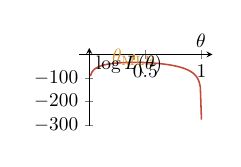
\begin{tikzpicture}[scale=0.7]
    \begin{axis}[width=4cm, height=3cm, xlabel=$\theta$, ylabel={$\log L(\theta)$}, domain=0:1, samples=100, axis lines=middle, enlargelimits]
        \addplot[wp-primary, thick] {20*ln(x) + 30*ln(1-x)};
        \addplot[wp-accent, thick, dashed] coordinates {(0.4,0) (0.4, {20*ln(0.4)+30*ln(0.6)})};
        \node[wp-accent] at (0.4, -3) {$\hat{\theta}_{\text{MLE}}$};
    \end{axis}
\end{tikzpicture}
\caption{Log‑likelihood for a Binomial experiment (20 successes, 30 failures); the MLE is $\hat{\theta}=0.4$.}
\end{marginfigure}

\paragraph{Connection to Empirical Risk Minimization}
For many models, MLE is equivalent to minimizing a specific loss function. For example:
\begin{itemize}
    \item \textbf{Linear regression with Gaussian noise:} $y = \mathbf{w}^{\mathsf{T}}\mathbf{x} + \varepsilon$, $\varepsilon \sim \mathcal{N}(0,\sigma^2)$. The negative log‑likelihood is proportional to the squared loss: $-\log p(\mathbf{y} \mid \mathbf{X}, \mathbf{w}) = \frac{1}{2\sigma^2}\sum_i (y_i - \mathbf{w}^{\mathsf{T}}\mathbf{x}_i)^2 + \text{const}$.
    \item \textbf{Binary classification with logistic model:} $p(y=1 \mid \mathbf{x}) = \sigma(\mathbf{w}^{\mathsf{T}}\mathbf{x})$. The negative log‑likelihood gives the binary cross‑entropy loss.
\end{itemize}
Thus, minimizing empirical risk with appropriate loss functions corresponds to MLE.

\subsection{Properties of MLE}

Under regularity conditions (e.g., the Fisher information matrix is positive definite), the MLE enjoys several asymptotic properties:

\begin{thm}[Consistency]
    As $N \to \infty$, $\hat{\boldsymbol{\theta}}_{\text{MLE}} \xrightarrow{P} \boldsymbol{\theta}_0$, where $\boldsymbol{\theta}_0$ is the true parameter.
\end{thm}

\begin{thm}[Asymptotic Normality]
    \[
    \sqrt{N}\bigl(\hat{\boldsymbol{\theta}}_{\text{MLE}} - \boldsymbol{\theta}_0\bigr) \xrightarrow{d} \mathcal{N}\bigl(\mathbf{0}, \mathcal{I}(\boldsymbol{\theta}_0)^{-1}\bigr),
    \]
    where $\mathcal{I}(\boldsymbol{\theta}_0) = \mathbb{E}\bigl[-\nabla^2_{\boldsymbol{\theta}}\log p(\mathbf{x},y;\boldsymbol{\theta}_0)\bigr]$ is the Fisher information matrix.
\end{thm}

These properties justify the widespread use of MLE: for large sample sizes, it is efficient (lowest possible variance among unbiased estimators) and approximately Gaussian.

\subsection{Bayesian Inference}

Bayesian inference treats the parameter $\boldsymbol{\theta}$ itself as a random variable, encoding prior beliefs before seeing the data.

\begin{defn}[Bayes' Theorem for Parameters]
    Given a prior distribution $\pi(\boldsymbol{\theta})$ and likelihood $L(\boldsymbol{\theta}; \mathcal{D}) = p(\mathcal{D} \mid \boldsymbol{\theta})$, the posterior distribution is
    \[
    p(\boldsymbol{\theta} \mid \mathcal{D}) = \frac{p(\mathcal{D} \mid \boldsymbol{\theta}) \, \pi(\boldsymbol{\theta})}{p(\mathcal{D})},
    \qquad p(\mathcal{D}) = \int p(\mathcal{D} \mid \boldsymbol{\theta}) \pi(\boldsymbol{\theta})\,d\boldsymbol{\theta}.
    \]
\end{defn}

The posterior combines prior knowledge with evidence from the data. Predictions for a new input $\mathbf{x}_{\text{new}}$ are made via the \textbf{posterior predictive distribution}:
\[
p(y_{\text{new}} \mid \mathbf{x}_{\text{new}}, \mathcal{D}) = \int p(y_{\text{new}} \mid \mathbf{x}_{\text{new}}, \boldsymbol{\theta}) \, p(\boldsymbol{\theta} \mid \mathcal{D}) \, d\boldsymbol{\theta}.
\]

\begin{marginfigure}
\centering
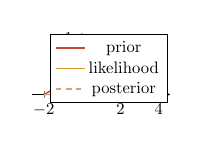
\begin{tikzpicture}[scale=0.6]
    \begin{axis}[width=4.5cm, height=3cm, xlabel=$\theta$, ylabel=density, domain=-2:4, samples=100, axis lines=middle, enlargelimits]
        \addplot[wp-primary, thick] {exp(-(x+0.5)^2/0.5)}; % prior
        \addplot[wp-accent, thick] {exp(-(x-1.5)^2/0.2)}; % likelihood
        \addplot[wp-muted, thick, dashed] {exp(-(x-0.8)^2/0.15)}; % posterior
        \legend{prior, likelihood, posterior};
    \end{axis}
\end{tikzpicture}
\caption{Prior, likelihood, and posterior. The posterior shrinks toward the likelihood when data are informative.}
\end{marginfigure}

\subsection{Conjugate Priors}

A prior is \textbf{conjugate} to a likelihood family if the posterior belongs to the same family as the prior. This simplifies computation and allows closed‑form updates.

\begin{exmp}[Beta–Binomial Conjugacy]
    For binary data $y_i \sim \text{Bernoulli}(\theta)$, the conjugate prior is the Beta distribution: $\pi(\theta) = \text{Beta}(\alpha, \beta)$. The posterior is $\text{Beta}(\alpha + \sum y_i,\; \beta + N - \sum y_i)$.
\end{exmp}

\begin{exmp}[Normal–Normal Conjugacy]
    For data $x_i \sim \mathcal{N}(\mu, \sigma^2)$ with known variance $\sigma^2$, a conjugate prior on $\mu$ is $\mu \sim \mathcal{N}(\mu_0, \tau_0^2)$. The posterior is Gaussian with updated mean and variance.
\end{exmp}

\subsection{Relation to Regularization}

Maximum a posteriori (MAP) estimation finds the mode of the posterior:
\[
\hat{\boldsymbol{\theta}}_{\text{MAP}} = \arg\max_{\boldsymbol{\theta}} \log p(\mathcal{D} \mid \boldsymbol{\theta}) + \log \pi(\boldsymbol{\theta}).
\]
The log‑prior term acts as a regularizer. For example:
\begin{itemize}
    \item Gaussian prior $\pi(\boldsymbol{\theta}) \propto \exp(-\lambda \|\boldsymbol{\theta}\|_2^2)$ induces L2 regularization (ridge regression).
    \item Laplace prior $\pi(\boldsymbol{\theta}) \propto \exp(-\lambda \|\boldsymbol{\theta}\|_1)$ induces L1 regularization (LASSO).
\end{itemize}
Thus, Bayesian inference provides a probabilistic justification for common regularization techniques used in deep learning.

\subsection{Challenges and Approximations for Deep Learning}

Exact Bayesian inference is intractable for large neural networks due to the high‑dimensional integral over parameters. Practical deep learning uses approximations:
\begin{itemize}
    \item \textbf{Variational inference:} approximate the posterior with a tractable distribution $q_{\boldsymbol{\phi}}(\boldsymbol{\theta})$ by minimizing $D_{\text{KL}}(q \parallel p)$.
    \item \textbf{Monte Carlo dropout:} interpreting dropout as approximate Bayesian inference (Gal \& Ghahramani, 2016).
    \item \textbf{Laplace approximation:} Gaussian approximation around the MAP estimate.
    \item \textbf{Stochastic gradient MCMC:} sampling methods like SGLD (stochastic gradient Langevin dynamics).
\end{itemize}

These approximations enable uncertainty quantification in deep learning, a critical ingredient for reliable decision‑making.

\begin{marginfigure}
\centering
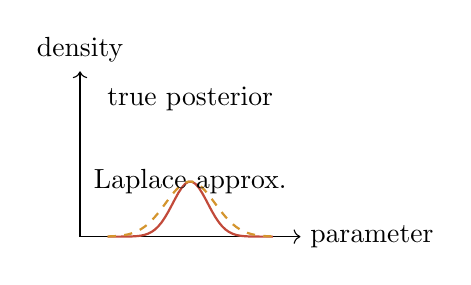
\begin{tikzpicture}[scale=0.7]
    \draw[->] (0,0) -- (4,0) node[right] {parameter};
    \draw[->] (0,0) -- (0,3) node[above] {density};
    \draw[wp-primary, thick, domain=0.5:3.5, samples=50] plot (\x, {exp(-(\x-2)^2/0.2)});
    \draw[wp-accent, thick, dashed, domain=0.5:3.5, samples=50] plot (\x, {exp(-(\x-2)^2/0.4)});
    \node at (2,2.5) {true posterior};
    \node at (2,1) {Laplace approx.};
\end{tikzpicture}
\caption{Laplace approximation: a Gaussian centered at the MAP estimate.}
\end{marginfigure}

With MLE and Bayesian inference established, we have a complete probabilistic framework that unifies loss functions, regularization, and uncertainty quantification – all essential for understanding deep learning from first principles.


\bibliographystyle{plain}
\begin{thebibliography}{1}
\bibitem{Vapnik1998} V. Vapnik, \textit{Statistical Learning Theory}. Wiley-Interscience, 1998.
\bibitem{Bishop2006} C. M. Bishop, \textit{Pattern Recognition and Machine Learning}. Springer, 2006.
\end{thebibliography}

\end{document}